\section{Funzione generatrice}

\setcounter{equation}{0}

Torniamo ora a $\mathcal{V}_{n+1}$ e a $T^* (\mathcal{V}_{n+1})$. Le considerazioni precedenti si riportano a questo contesto restringendo l'attributo di \textit{canonico} ai sistemi di coordinate \\
\label{pag_funz_gen}
\begin{equation*}
	x^1, \dots ,x^m, y_1, \dots , y_n \equiv q^0, q^1, \dots , q^n, P_0, P_1, \dots , P_n
\end{equation*}
che, oltre a dare luogo alla \textit{rappresentazione} della $ 2 $-forma simplettica nella forma
\begin{equation*}
	\Omega(X, Y) = \sum_{\alpha = 0}^n \left( \langle dP_{\alpha}, X \rangle \langle dq^{\alpha}, Y \rangle - \langle dq^{\alpha}, X \rangle \langle dP_{\alpha}, Y \rangle \right)
\end{equation*}

\begin{equation*}
	\left( \iff \Omega(X, Y) = \sum_{\alpha = 0}^{n} X_{\alpha} Y^{\alpha} - X^{\alpha} Y_{\alpha} \right)
\end{equation*}

\begin{align*}
	X &= X^{\alpha} \frac{\partial}{\partial q^{\alpha}} + X_{\alpha} \frac{\partial}{\partial P_{\alpha}} \\
	Y &= Y^{\alpha} \frac{\partial}{\partial q^{\alpha}} + Y_{\alpha} \frac{\partial}{\partial P_{\alpha}}
\end{align*}
\textit{sussista l'identificazione} $q^o \equiv t$. \, $( t = \text{tempo} )$.

\begin{center}
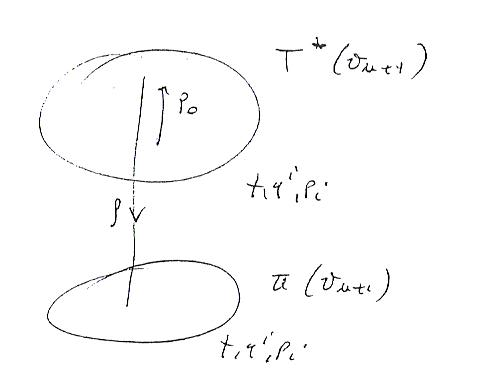
\includegraphics[width=0.5\columnwidth]{media/funzione-generatrice/32-1.jpg}
\end{center}

Le trasformazioni canoniche in $T^* (\mathcal{V}_{n+1})$ saranno quelle che preservano la rappresentazione della $2$-forma simplettica di $T^* (\mathcal{V}_{n+1})$ insieme all'identificazione $q^0 = t$ (cioè $q^{0'} = t' = t$ nelle nuove coordinate).

Avendo in mente la caratterizzazione delle trasformazioni canoniche data a pagina $\pageref{pag:trasf_can_pag24}$ in termini di una funzione generatrice, che ora chiamiamo $ \tilde{F} = \tilde{F} (t, q^1, \dots , q^n, P'_0, P'_1, \dots , P'_n) $, abbiamo
\begin{align*}
	q'^0 &= \frac{\partial \tilde{F}}{\partial P'_0} (t, q^1, \dots , q^n, P'_0, P'_1, \dots , P'_n) \\
	q'^i &= \frac{\partial \tilde{F}}{\partial P'_i} (t, q^1, \dots , q^n, P'_0, P'_1, \dots , P'_n) \\
	P_0 &= \frac{\partial \tilde{F}}{\partial t} (t, q^1, \dots , q^n, P'_0, P'_1, \dots , P'_n) \\
	P_i &= \frac{\partial \tilde{F}}{\partial q^i} (t, q^1, \dots , q^n, P'_0, P'_1, \dots , P'_n)
\end{align*}

Vediamo subito che la condizione $ q^{0'} = t' = t = q^0 $ implica
\begin{equation*}
	t' = \frac{\partial \tilde{F}}{\partial P'_0} = t
\end{equation*}
da cui
\begin{equation*}
	 \tilde{F} (t, q^1, \dots , q^n, P'_0, P'_1, \dots , P'_n) = P'_0 \cdot t + F (t, q^1, \dots , q^n, P'_0, P'_1, \dots , P'_n)
\end{equation*}
(da qui in avanti, dato l'uso frequente, chiameremo con $ F $ la parte di $ \tilde{F} $ depurata di $ P'_0 \cdot t $ (la $ F $ introdotta ora, evidentemente, \textit{non} è la $ F $ introdotta a pagina $ \pageref{pag:trasf_can_pag24} $ )).

Pertanto abbiamo
\begin{equation*}
\begin{cases}
	t' = t\\
	q'^i = \frac{\partial F}{\partial P'_i}\\
	P_0 = P'_0 + \frac{\partial F}{\partial t}\\
	P_i = \frac{\partial F}{\partial q^i}
\end{cases}
	F = F (t, q^1, \dots , q^n, P'_1, \dots , P'_n)
\end{equation*}
dove $ F = F (t, q^1, \dots , q^n, P'_1, \dots , P'_n) $

% FINE PAGINA 32 - INIZIO PAGINA 33

Le relazioni
\begin{align*}
	q'^i &= \frac{\partial F}{\partial P'_i} (t, q^i, P'_i)\\
	P_i &= \frac{\partial F}{\partial q^i} (t, q^i, P'_i)
\end{align*}
esprimono, in forma implicita (ma esplicitabile ogniqualvolta sia soddisfatta la condizione
\begin{equation*}
	det \left( \frac{\partial^2 F}{\partial q^i \partial P'_j} \right) \neq 0
\end{equation*}
che assicura l'applicabilità del teorema della funzione inversa) la trasformazione canonica generata da $ F (t, q^i, P'_i) $, mentre la relazione
\begin{equation*}
	P_0 = P'_0 + \frac{\partial F}{\partial t}
\end{equation*}
fornisce, indirettamente, la legge di trasformazione della funzione Hamiltoniana. Rappresentata la superficie $ \Psi (j_1 (\mathcal{V}_{n+1})) = \Psi (\pi (\mathcal{V}_{n+1})) \subset T^* (\mathcal{V}_{n+1}) $ nella forma
\begin{equation*}
	P_0 + H = P'_0 + H' = 0
\end{equation*}
si deduce
\begin{equation*}
	H' = H + \frac{\partial F}{\partial t}
\end{equation*}

(Ovviamente, affinché i due membri di quest'ultima relazione siano effettivamente confrontabili, occorre che il secondo membro (ad esempio) venga espresso in termini delle variabili del primo, $ t, q', P' $, utilizzando la trasformazione di coordinate generata da $ F $).

Riprendiamo la formula data a pagina $ \pageref{pag:trasf_leg_geom} $ che esprime l'evoluzione lungo i moti (cioè lungo le soluzioni delle equazioni di Hamilton) di una generica funzione $ f: \pi (\mathcal{V}_{n+1}) \longrightarrow \mathbb{R} $

\begin{equation*}
	\frac{df}{dt} = \{f, P_0 + H (t, q, P) \} = \{f, P'_0 + H' (t, q', P') \}
\end{equation*}

(Le parentesi di Poisson qui coinvolte sono ovviamente quelle in $ T^* (\mathcal{V}_{n+1}) $, e la $ f $ va pensata come il pull-back a $ T^* (\mathcal{V}_{n+1}) $ della $ f $ definita su $ \pi (\mathcal{V}_{n+1}) $).

\begin{equation*}
	\frac{df}{dt} = \{f, P'_0 \} + \{f, H' \} = \frac{df}{dt} + \frac{df}{dq'^i}\frac{dH'}{dP'_i} - \frac{df}{dP'_i}\frac{dH'}{dq'^i}
\end{equation*}
ovvero, in particolare, quando $ f = q'^i $ e $ f = P'_i $
\begin{align*}
	\frac{dq'^i}{dt} &= \frac{\partial H'}{\partial P'_i}\\
	\frac{dP'_i}{dt} &= - \frac{\partial H'}{\partial q'^i}
\end{align*}
ovvero, $ Z = \frac{\partial}{\partial t} + \frac{\partial H'}{\partial P'_i} \frac{\partial}{\partial q'^i} - \frac{\partial H'}{\partial q'^i} \frac{\partial}{\partial P_i} $
il che mostra \textit{l'invarianza in forma delle equazioni di Hamilton per effetto di una trasformazione canonica}.
